\documentclass{article}

\usepackage{graphicx}
\usepackage{tikz}
\usepackage{tikzsymbols}
\usetikzlibrary{calc,patterns,shapes.geometric}
\pagestyle{empty}
\usepackage[margin=0pt]{geometry}
\geometry{papersize={14in,12in}}

\def\centerarc[#1](#2)(#3:#4:#5){\draw[#1] ($(#2)+({#5*cos(#3)},{#5*sin(#3)})$) arc (#3:#4:#5);}

\begin{document}
	\begin{figure}
		\centering
		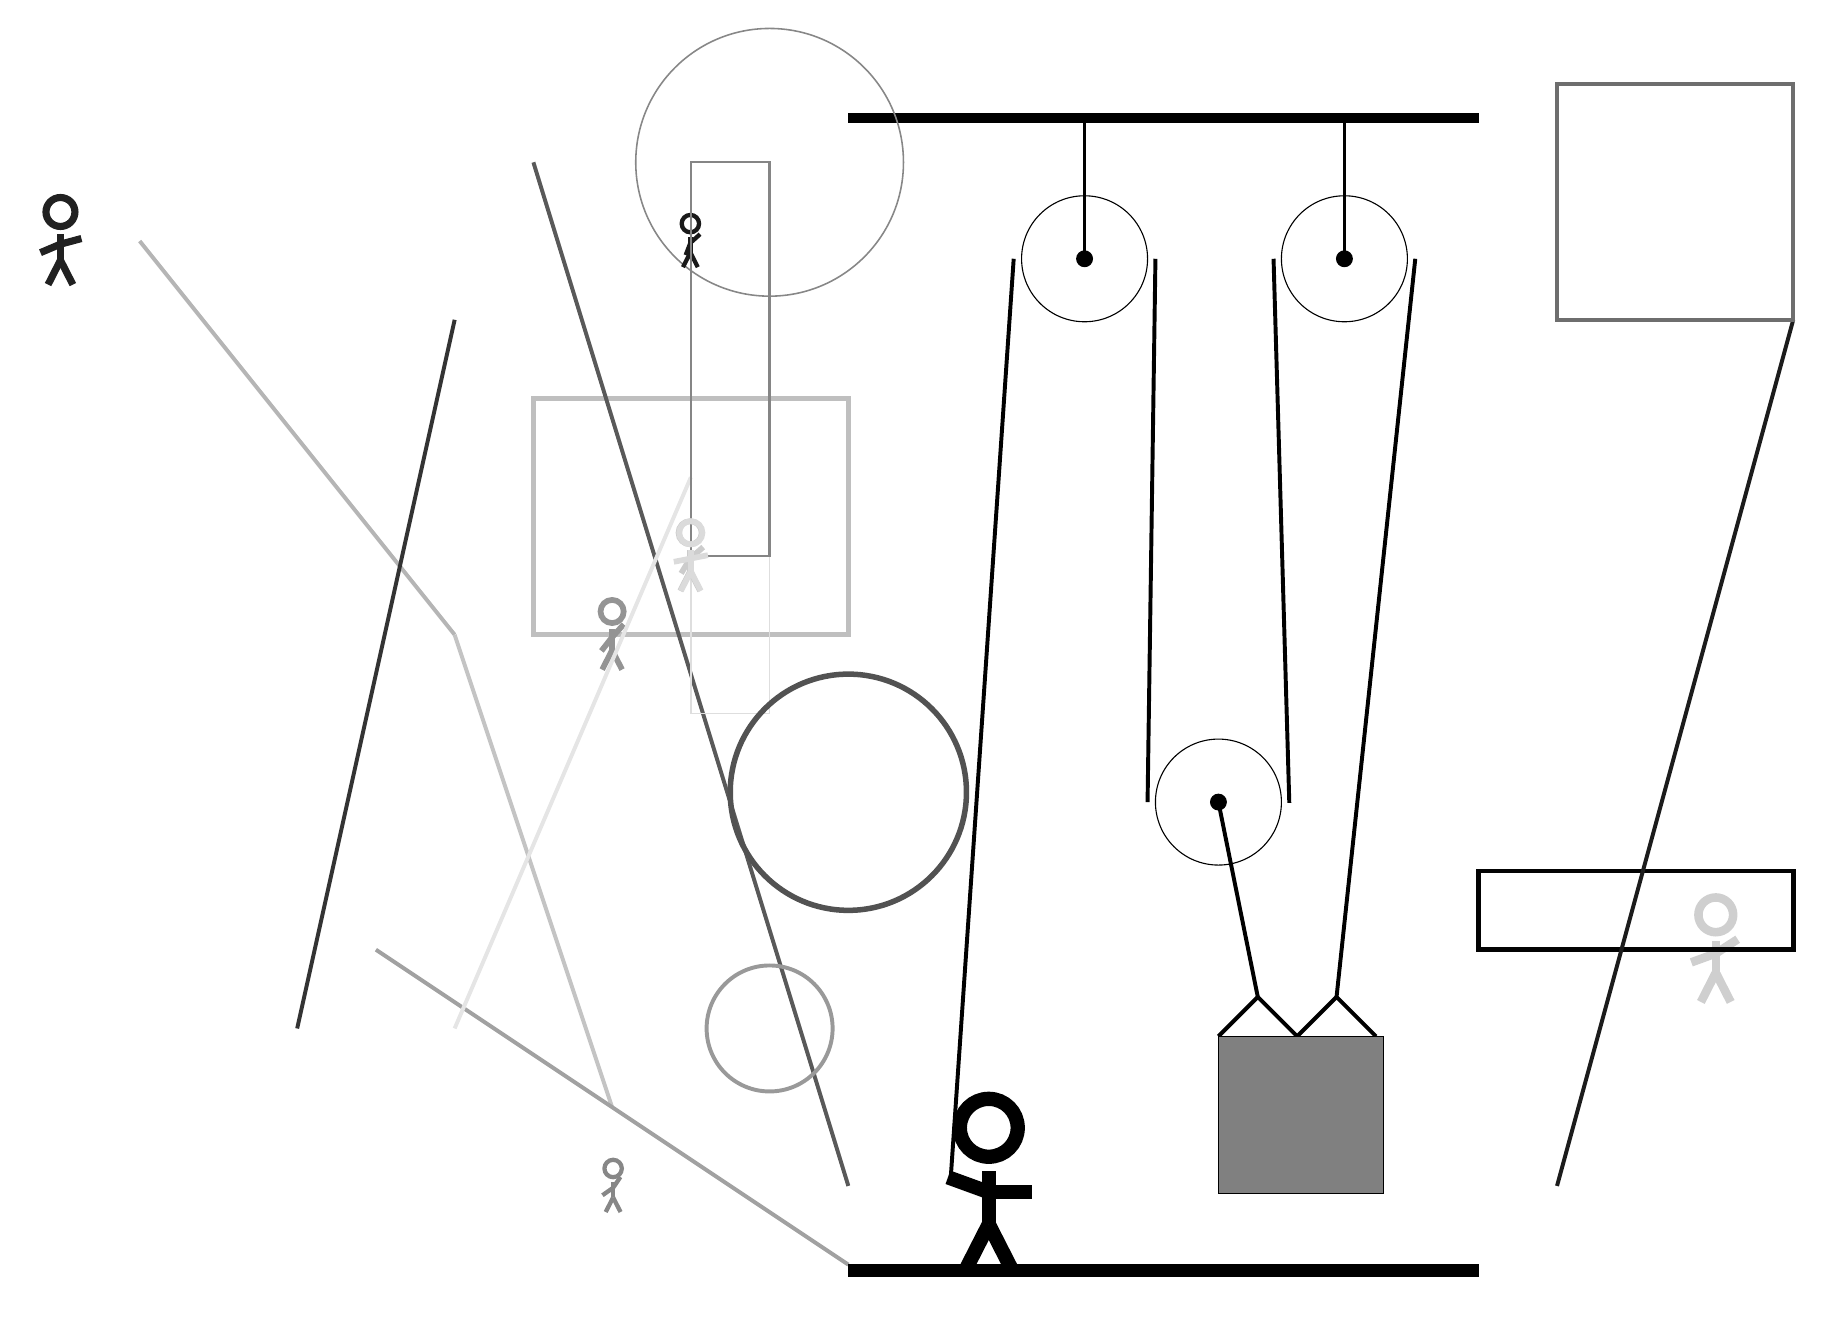
\begin{tikzpicture}
			%%%%% START %%%%%
			
			\draw[fill=black] (-2, 11.5) rectangle (6, 11.625);
			
			\draw (1, 9.775) circle (0.8);
			\draw[fill=black] (1, 9.775) circle (0.1);
			\draw[thick] (1, 9.775) -- (1, 11.5);
			
			\draw (4.3, 9.775) circle (0.8);
			\draw[fill=black] (4.3, 9.775) circle (0.1);
			\draw[thick] (4.3, 9.775) -- (4.3, 11.5);
			
			\draw (2.7, 2.875) circle (0.8);
			\draw[fill=black] (2.7, 2.875) circle (0.1);
			
			\draw[line width=0.5mm]  (2.7, -0.1) -- (3.2, 0.4) -- (3.7, -0.1) -- (4.2, 0.4) -- (4.7, -0.1);
			\draw[fill=black!50] (2.7, -0.1) rectangle (4.8, -2.1);
			
			\draw[line width=0.5mm](-0.7, -1.9) -- (0.1, 9.775);
			\centerarc[line width=0.5mm](1, 9.775)(0:180:0.9);
			\draw[line width=0.5mm](1.9, 9.775) -- (1.8, 2.875);
			\centerarc[line width=0.5mm](2.7, 2.875)(180:370:0.9);
			\draw[line width=0.5mm] (3.6, 2.865) -- (3.4, 9.775);
			\centerarc[line width=0.5mm](4.3, 9.775)(0:180:0.9);
			\draw[line width=0.5mm](4.2, 0.4) -- (5.2, 9.775);
			\draw[line width=0.5mm] (3.2, 0.4) -- (2.7, 2.875);
			
			\draw[line width=0.6mm, color=black!25] (-2, 5) rectangle (-6, 8);
			
			\draw[line width=0.5mm, color=black!65](-2, -2) -- (-6, 11);
			\node[line width=0.3mm, color=black!19] at (9, 1) {\Strichmaxerl[6][20][33]};
			\draw[line width=0.2mm, color=black!13] (-3, 11) rectangle (-4, 4);
			\draw [line width=0.5mm, color=black!40](-3, 0) circle (0.8);
			\node[line width=0.5mm, color=black!42] at (-5, 5) {\Strichmaxerl[4][52][48]};
			\draw[line width=0.5mm, color=black!29](-7, 5) -- (-11, 10);
			
			\draw[line width=0.6mm, color=black!99] (6, 1) rectangle (10, 2);
			\draw[line width=0.5mm, color=black!23](-7, 5) -- (-5, -1);
			
			\draw[line width=0.5mm, color=black!37](-2, -3) -- (-8, 1);
			\draw [line width=0.2mm, color=black!47](-3, 11) circle (1.7);
			
			\node[line width=0.7mm, color=black!90] at (-4, 10) {\Strichmaxerl[3][69][42]};
			\node[line width=0.7mm, color=black!47] at (-5, -2) {\Strichmaxerl[3][35][56]};
			\draw[line width=0.5mm, color=black!10](-7, 0) -- (-4, 7);
			\draw[line width=0.3mm, color=black!48] (-4, 6) rectangle (-3, 11);
			\node[line width=0.4mm, color=black!87] at (-12, 10) {\Strichmaxerl[5][23][15]};
			\node[line width=0.4mm, color=black!20] at (-4, 6) {\Strichmaxerl[4][59][41]};
			\draw[line width=0.5mm, color=black!89](10, 9) -- (7, -2);
			\node[line width=0.7mm, color=black!14] at (-4, 6) {\Strichmaxerl[4][11][11]};
			\draw [line width=0.7mm, color=black!68](-2, 3) circle (1.5);
			\draw[line width=0.5mm, color=black!80](-7, 9) -- (-9, 0);
			\draw[line width=0.5mm, color=black!57] (7, 12) rectangle (10, 9);
			
			
			\node at (-0.2, -2) {\Strichmaxerl[10][-20][0]};
			
			\draw[fill=black] (-2, -3) rectangle (6, -3.15);
			
			%%%%% END %%%%%
		\end{tikzpicture}
	\end{figure}	
\end{document}